% !TeX root = ../../master_thesis.tex

\section{Conversational banking}

Conversational banking is a revolution in bank interaction with clients.
This term is comparably new and represents an approach in the bank interaction of banks with their customers in their natural language through a dialogue interface or special widgets, which makes dialog more comfortable.

People change their behavior and habits in favor of dialog interfaces, as they wait fast and qualified answers.
One specialist sometimes may not promptly respond to a client request and needs a pause, in order to either find and answer or transfer request to a more experienced specialist.
In this case client has to wait, sometimes for a long time, which can create irritation and, respectively, decrease the level of satisfaction.

One of the leaders of market of professional services in digital technologies, Accenture, in its researches found out that existing online interaction channels are gradually becoming obsolete.
Therefore, banks have to use a brand-new way, by establishing a continuous conversation, in order to eliminate the flaws of models used on a current stage of banking technologies development.
Digital platforms are extremelly important for banks.
\cite{accenture_conversational_banking}

\begin{figure}
    \centering
    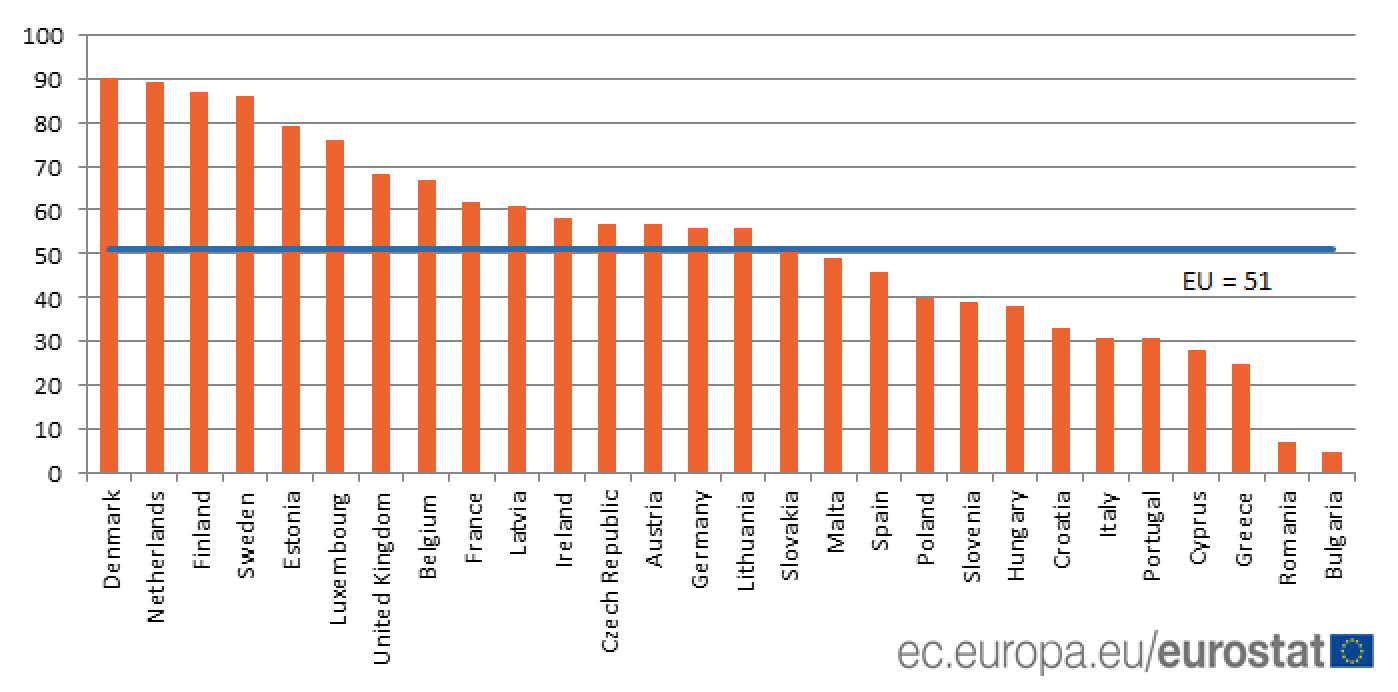
\includegraphics[width=0.8\textwidth,height=\textheight,keepaspectratio]{images/share_internet_banking.png}
    \caption{\% of individuals who used internet banking}
    \medskip
    \footnotesize\textit{Source:} "Individuals using the internet for internet banking", Eurostat, 2021.
\end{figure}

By 2017, 51\% of bank customers in European Union used internet and mobile banking at least once.
And based on the latest trends and situations, the share of internet banking will only grow.
Consequently, consumer banks are interested in offering major services via digital channels, and to research and develop modern solutions.
However, the main interest is in creating modern, and at the same time, comfortable and usual channel for user interaction, and, especially, for two-way user communication.

Obviously, the closest form of such interaction to live communication would be a form of questions and answers.
This form of interaction became widely popular due to search engines and its influence on an internet for the last decade.

People of all generations are used to asking questions on digital platforms.
Search engines have been actively developing and implementing technologies related to operating with natural languages for the last ten years.
Same engines have been studying internet users to write proper search queries to obtain expected results for decades.

\begin{figure}
    \centering
    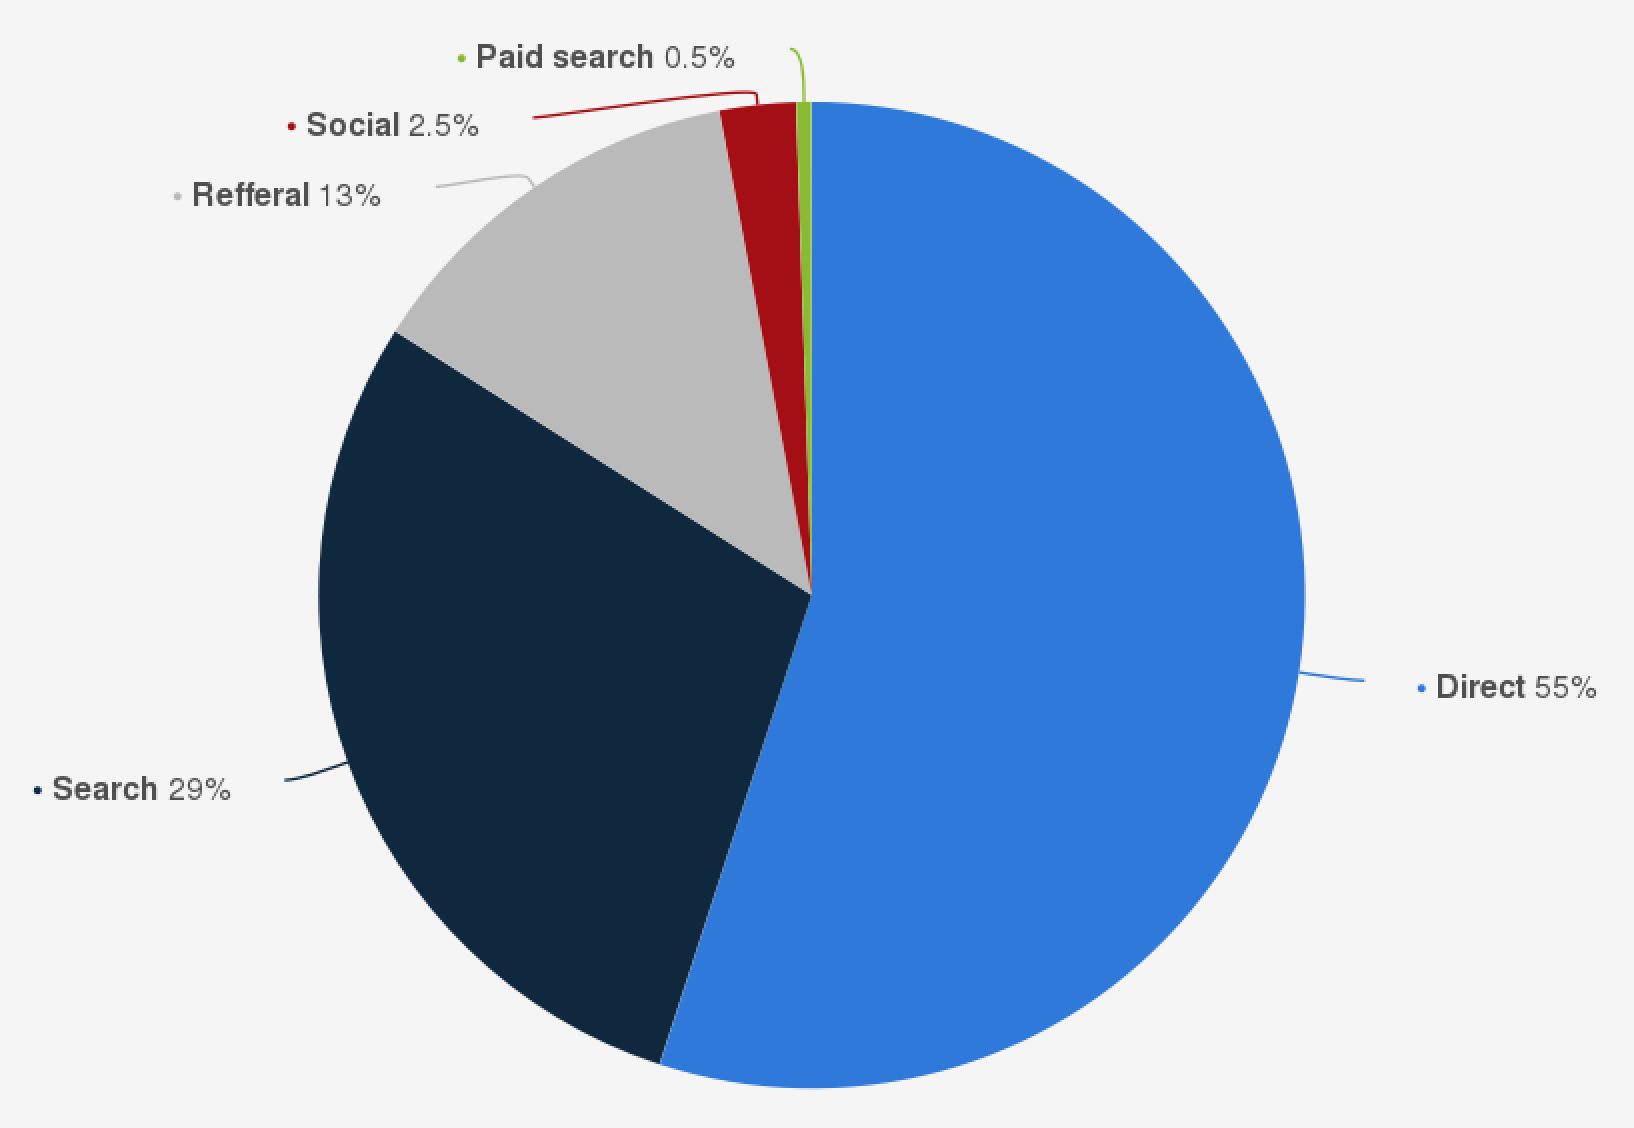
\includegraphics[width=0.8\textwidth,height=\textheight,keepaspectratio]{images/statista_search_engines.png}
    \caption{Distribution of worldwide search traffic}
    \medskip
    \footnotesize\textit{Source:} Jessica Clement "Global website traffic distribution", Statista, 2019.
\end{figure}

Nowadays, search engines have nearly 30\% of entire internet traffic.
Without ten most popular non-search engine websites this share would be around 90\%.
The influence of search engines on conversation technologies is impossible to overstate.
What is even more important, for the last ten years those technologies have been in active development and deployment, resulting in existance of a stable branch of technology with a lot of modern solutions.

Natural Language Processing is a cognitive branch of science, that investigates the application of computational techniques to the analysis and synthesis of natural language and speech.
Natural Language Processing, known as NLP, consists of Natural Language Understanding, NLU, which analysis text and finds logical points and meaning, and Natural Language Generation, NLG, which structures, plans and generates human-readable text.
Generally, NLP, both Understanding and Generation, including Voice Synthesis, became a pretty common part of technology for a user, especially due to Voice Assistants.
What is even more important, for the last ten years the cost of implementation of mentioned technologies significantly decreased.
On the contrary, amounts of investements into AI and NLP drastically increase every year.
In 2020 global NLP market value was \$1.8 billion, and is expected to grow up to \$14.4 billion by 2026.
\cite{pwc_ai_nlp}

\begin{figure}
    \centering
    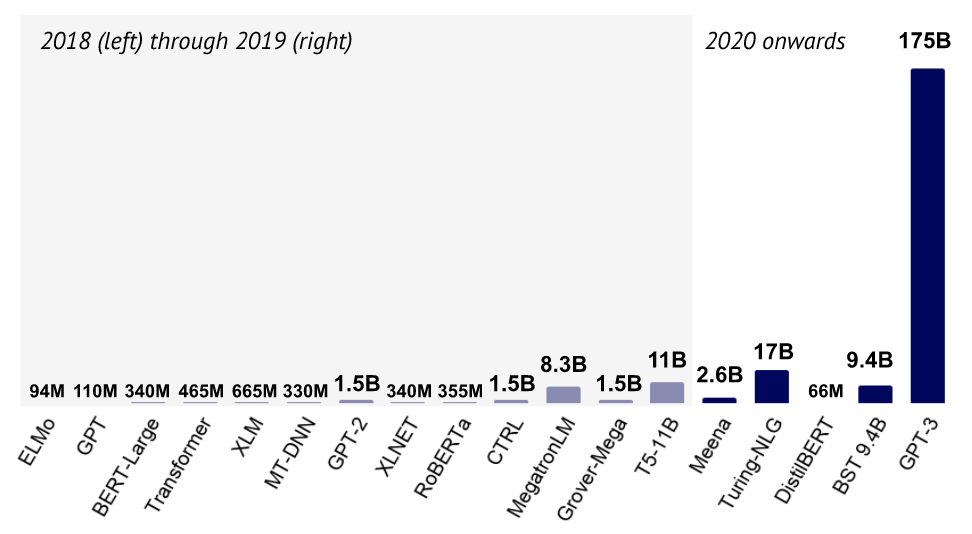
\includegraphics[width=0.8\textwidth,keepaspectratio]{images/nlp_models_parameters.png}
    \caption{Number of parameters in NLP AI algorithms}
    \medskip
    \footnotesize\textit{Source:} Nathan Benaich, Ian Hogarth "State of AI Report", stateofai.com, 2020, s. 15.
\end{figure}

It is important to highlight the exponential grow and compliction of those models. 
NLP models can have multiple billions of parameters and coefficients, that those use for text analysis and generation, with a current record of 175 billion parameters by famous GPT-3.

Main purpose of NLP with AI in this case is to replace usual contact centers and to improve customer experience.
The reason of replacement is a comparingly low conversion for existing solutions.
Contact centers are infamous for response times and low quality of solutions.
This is extremelly important, as consumers have low conversion rates if brands don't answer phone in under a minute.
Based on researches, 78\% of responsers may switch brand preferences due to poor response times, while 73\% will recommend highly responsive brands.
Additionally, 59\% of responders have extremelly high conversion rate for highly responsive brands.
\cite{lfbyphone_consumer_analytics}

At the same time, achieving positive feedback in under a minute is a main target of automated conversational banking.
Chat-bots are known for giving high conversion rates and large returns on considerable small inverstments.
\cite{accenture_ai_banking}

In consequence, banks can strive to major influence of dialog interfaces on client, through which clients can transfer funds, send it to other clients, issue card, convert currency, execute payments and various other basic tasks.

It is common to mix up Conversational banking with Mobile and Internet Banking.
However, the main difference is in user experience.
Mobile and Internet banking are hierarchical trees, both of those have a concrete form.
It is always an application, in which user can click buttons, check charts and read text in order to manipulate and make actions.
Conversational banking is much more abstract.
That is a dialog, client should not in this case know the structure of interaction.
In order to achieve something client has to have an intent and, what is even more important, to invoke an action by intention.
He doesn't need to know how to achieve something, he can just ask.
However, in this case client can rely only on his knowledge, as there would be no buttons or menus to check.

Front-office for Conversational banking may have different forms.
This can be a contact center, retail business unit for dialog-based conversation.
Couple of years ago, bank client on any problem had to call to a contact center and to talk to customer service line manager. 
\cite{trillion_opportunity}
Nowadays, there are other options.
Much more interesting option is a messenger, as a front-office for textual interactions.
In this case, this can be both a chat-bot in a popular messenger app or a social network, same chat-bot in a mobile or internet banking app, or even a voice assistant.

Currently, it is a popular solution to use chat-bots which can answer to the most simple question, but mostly transfer a conversation to the contact center.
Though, this is a not a most effective model, as client firstly has to spend his time to describe his problem to a chat-bot, and then he has to repeat to a human specialist.
\cite{accenture_conversational_banking}

\begin{table}
    \centering
    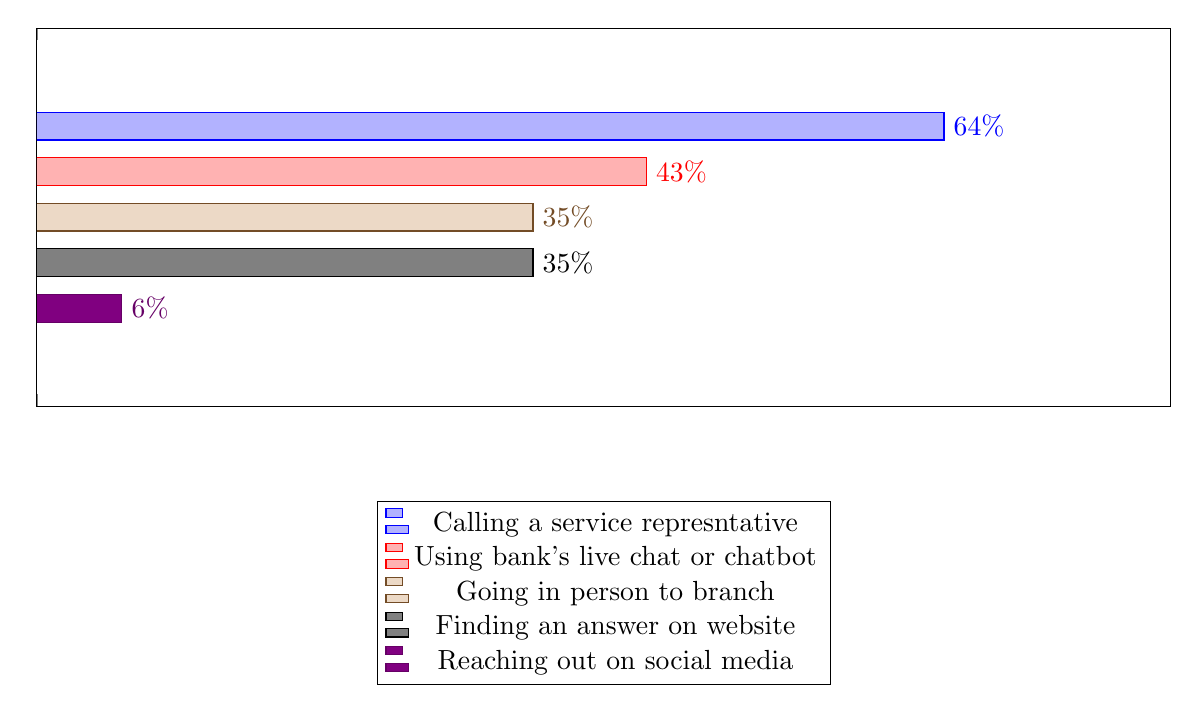
\begin{tikzpicture}
        \begin{axis} [
            xbar,
            xmin=0, xmax=80,
            x=0.18cm, y=1cm,
            xticklabels={,,},
            yticklabels={,,},
            xtick = {0}, ytick = \empty,
            nodes near coords,
            nodes near coords style={ anchor=west },
            point meta=explicit symbolic,
            legend style={at={(0.5,-0.25)},anchor=north}
        ]

        \addplot coordinates {(64,4)[64\%]};
        \addplot coordinates {(43,3)[43\%]};
        \addplot coordinates {(35,2)[35\%]};
        \addplot coordinates {(35,1)[35\%]};
        \addplot coordinates {(6,0)[6\%]};

        \legend{
            Calling a service represntative, 
            Using bank's live chat or chatbot,
            Going in person to branch,
            Finding an answer on website,
            Reaching out on social media
        }
        \end{axis}
    \end{tikzpicture}
    \caption{Consumer preferences for addressing issues}
    \medskip
    \footnotesize
    \textit{Source:} Own study, based on Bill Streeter "Banking By Bot: Are Chatbots Better Than Real People?", The Financial Brand, 2018
\end{table}
    
However, for customer it is still more comfortable to address problems via common channels of interactions, such as via phone calls or via in-person conversation in a branch.
\cite{humley_banking_report}

This is due too negative experience with current automated conversational solutions.
It is too early to talk about conversational banking in a poor form, as chat-bots are on such level of development, that those cannot be used purely, as they don't understand all the requests yet.
This results in a negative influence towards client satisfaction.

On the other side, it is important to discuss approaches to build this system.
During client conversation it is important to transfer from screen interface of mobile or internet-bank to creation of universal and operational assistant, which would be ready to interact and to help a client at any time.
This form of client interaction is based on an understanding of a global trend, as more and more people are used to talk with sellers via messengers.
Even though automated solutions are not common, those, nearly 44\% of customers would prefer to speak to chatbot, if they are sure, that a chat-bot knows an answer.
\cite{humley_banking_report}
Therefore, implementing any automatized conversational interface for a bank is impossible without influencing expectations.
This transforms entire service consumption process, as it is more comfortable to contact via suitable and familiar solutions and messengers.

Conversational banking has some significant advantages in comparison to existing systems.
Firstly, improvement of client experience. 
We can make it more comfortable, fast and qualified.
Secondly, conversational banking decreases client waiting time. 
If chat-bot is not sure about the question or the answer, dialog can be transferred to a human operator.
In case if system achieves certain level of assurance — it will reply automatically.
Researches of client experience had shown that verbal interaction is psychologically more comfortable and brings less cognitive load than visual interface.
\cite{accenture_conversational_banking}

From a practical perspective, conversational banking exists in two pure forms.
First form is a chat-bot, an automatic solution for textual communication with a client in a form of a dialog window.
The input in this case is a text provided by a user, and the output is a text returned by an analytical system, which consumes request and generates response.
Second form is a voice assistant. Internal work is analogical to a chat-bot, but it differs in a form of interaction.
Voice assistant receives spoken user messages and answers with synthesized voice responses.
Both of those forms are well known to users.
However, in most cases those are usually used as a support part and do not have sufficient level of autonomy.
Application of AI to those well known forms of interaction is the main purpose of Conversational Banking.

Consumers are used to chat and for them, it is easier than to click out their problem in an interface of website or mobile app.
The process of automation in banks is gradually growing and this, from the one side, should lead to a reduction of a number of contact center specialists.
On the other side, increasing number of customers consequently increases chat loads.
Nevertheless, increasing load shows higher client involvement.

Nonetheless, current state of AI application in Front-office has certain problems.
As it was mentioned before in \ref{subsec:ai_front_office}, conversational banking is not considered as available by middle-sized and small banks.
Mostly it is used either by the largest commercial banks, which have large amounts of resources available for investments, or by start-ups and new digital financial services, which are targeting market by innovations.

As a result, banks face a choice — use existing solutions or to create their own product, which is not available to small-sized and medium banks.
However, it is not entirely correct, as medium-sized and small banks can and have to use third-party solutions for implementation.
On the other hand, integration of external technologies uses very large volume of bank resources, as well as cost of product usage.
As a result, final cost may be higher than cost of internal development.

Another major problem is obvious and connected to existing employees in customer experience offices.
As cost decrease on customer support being a valid reason for banks, this doesn't mean that banks will decrease amount of support agents.
In contrast, those may be moved to other branches or to other banking products.
Additionally, support agents may require training for changing their profile.
The point of this action is not to decrease a number of employees, but to create a higher percentage of professionals among existing specialists.

\subsection{Hybrid approach}

Nevertheless, the largest banks already have solutions for dialog interfaces in messengers.
In those case, they are developing solutions for artificially augmented intellegence in client support.
It is a common misconception, that those chat-bots are for customers only.
Indeed, those are much more useful for bank employees as a single source of knowledge and can significantly improve client experience.
It is too early to talk about conversational banking in a poor form.

On other side, it is important to discuss approaches to build this system.
During client conversation it is important to transfer from screen interface of mobile or internet-bank to creation of universal and operational assistant, which would be ready to interact and to help a client at any time.
This form of client interaction is based on an understanding of a global trend, as more and more people are used to talk with sellers via messengers. 
This transforms entire service consumption process, as it is more comfortable to contact via suitable and familiar solutions and messengers.
Conversational banking has some significant advantages in comparison to existing systems.

Firstly, improvement of client experience. 
We can make it more comfortable, fast and qualified.
Secondly, conversational banking decreases client waiting time. If chat-bot is not sure about the question or the answer, dialog can be transferred to a human operator.
In case if system achieves certain level of assurance — it will reply automatically.
Researches of client experience had shown that verbal interaction is psychologically more comfortable and brings less cognitive load than visual interface.
Even the best market players warn — system should provide connection with a human, as there is no technology, that would allow delegating functions to computers entirely.
\cite{ways_ai_transforming_bi}

As well, chat-bot can answer by itself directly.
Unfortunately, currently it concerns only the most simple actions — customer welcoming, customer invitation, various forms of apologize, or informing the location of the nearest ATM.
If there is a large stream of clients, we can lower the system confidence threshold, in order to transfer clients to chat-bot, which could decrease waiting time and, as a result, increase client's service satisfaction.
Moreover, it is possible to involve one robot into dialogue with another robot.
For example, general support chat-bot can involve investment chat-bot.
\cite{accenture_chatbots}

\begin{figure}
    \centering
    \begin{tikzpicture}
        \begin{axis} [
            axis lines = middle,
            x axis line style={<->},
            smooth,
            xmin=-4, xmax=+4,
            ymin=55, ymax=92,
            xticklabels={,,},
            yticklabels={,,},
            xtick = \empty, ytick = \empty,
            ylabel = {Customer satisfaction rate},
            y label style={at={(axis description cs:0.5,1)},anchor=south},
            xlabel = {Conversion with\\Artificial Intelligence},
            x label style = {align = center, at={(axis description cs:1,0)},anchor=west},
            nodes near coords,
            nodes near coords style={ anchor=south west },
            point meta=explicit symbolic,
        ]

        \addplot+[mark=none] coordinates {
            (-4, 68)[68\%]
            (-1, 72)
            (0.1, 88)[88\%]
            (4, 60)[60\%]
        };

        \draw [dashed] (-4,68) -| (+4,68);
        \draw [dashed] (-4,88) -| (+4,88);
        \draw [dashed] (-4,60) -| (+4,60);

        \end{axis}
        
        \begin{axis} [
            axis y line = none,
            axis x line = bottom,
            xmin=-4, xmax=+4,
            ymin=55, ymax=92,
            xticklabels={,,}, yticklabels={,,},
            xtick = \empty, ytick = \empty,
            xlabel = {Conversion with\\alive agent},
            x label style = {align = center, at={(axis description cs:0,0)},anchor=east},
        ]
        \end{axis}
    \end{tikzpicture}
    \caption{Customer Satisfaction Rate by form of Live Chat}
    \medskip
    \footnotesize
    \textit{Source: Own study, based on "Chatbots are here to stay", Accenture, 2018}
\end{figure}

Conversational, dialog, bank is a hybrid between classic contact center and automated chat-bot service.
However, it is possible to use hybrid approach, in which robot recommends answer to an operator based on existing knowledge base.
Of course, the best possible answers are on top of the list, so it would be more comfortable for operator to find.
The best possible answer, in this case, would be an answer of the most competent expert, which would allow for an intern to answer on professional level.
Every client question and every operator answer are stored in database and is a template for future answers.
Operators are teachers and database is a student, and this is the way AI learns.
Of course, it requires specialists to develop such a system.

Similar augmentative system can be virtual broker, which give hints based on AI and can pick up an individual way to each client.
Nonetheless, there can be a personal-manager service, which communicates in chat and can execute large number of operations.
This may decrease loads, manual work, to transfer payments form from a manager to an AI.
Human-in-the-loop or HITL — a system, in which there should be a person for a proper functioning.
Specialist can choose various relevant actions.
Manager answers with text messages, as well as with special widgets with portfolio description or with operation confirmation. 
